% Source: TeX Live PGF manual, Coordinate Calculations / The General Syntax.
\documentclass[border=2pt]{standalone}
\usepackage{tikz}
\usetikzlibrary{calc}
\begin{document}
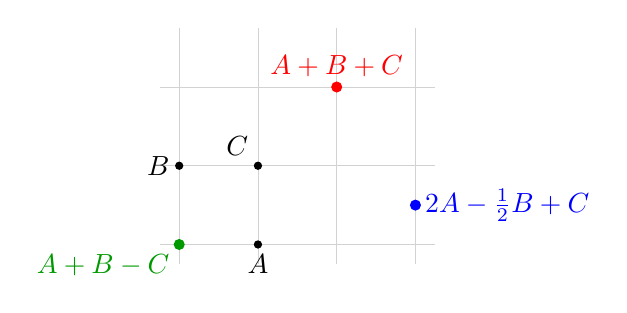
\begin{tikzpicture}
  \draw[help lines,gray!35] (-0.25,-0.25) grid (3.25,2.75);
  \coordinate (A) at (1,0);
  \coordinate (B) at (0,1);
  \coordinate (C) at (1,1);

  \fill (A) circle (1.5pt) node[below] {$A$};
  \fill (B) circle (1.5pt) node[left] {$B$};
  \fill (C) circle (1.5pt) node[above left] {$C$};

  \fill[red] ($(A)+(B)+(C)$) circle (2pt)
    node[above] {$A+B+C$};
  \fill[blue] ($2*(A)-.5*(B)+(C)$) circle (2pt)
    node[right] {$2A-\frac12B+C$};
  \fill[green!60!black] ($(A)+(B)-(C)$) circle (2pt)
    node[below left] {$A+B-C$};
\end{tikzpicture}
\end{document}
